%!TEX program = xelatex
\documentclass[11pt]{beamer}

\usepackage{amsfonts}
\usepackage{amsmath}
\usepackage{blindtext}
\usepackage{enumitem}
\usepackage{fancyvrb}

\usetheme{SaoPaulo}

\title{Python Basics!}
\subtitle{branched control, range, lists}
\author{CS101 Lecture \#8}
\date{2016-09-19}

\setcounter{showSlideNumbers}{1}

\begin{document}
  \setcounter{showProgressBar}{0}
  \setcounter{showSlideNumbers}{0}

%%%%%%%%%%%%%%%%%%%%%%%%%%%%%%%%%%%%%%%%%%%%%%%%%%%%%%%%%%%%%%%%%%%%%%%%%%%%%%%%
\frame{\titlepage}

%%%%%%%%%%%%%%%%%%%%%%%%%%%%%%%%%%%%%%%%%%%%%%%%%%%%%%%%%%%%%%%%%%%%%%%%%%%%%%%%
\setcounter{framenumber}{0}
\setcounter{showProgressBar}{1}
\setcounter{showSlideNumbers}{1}

%%%%%%%%%%%%%%%%%%%%%%%%%%%%%%%%%%%%%%%%%%%%%%%%%%%%%%%%%%%%%%%%%%%%%%%%%%%%%%%%
\section{Administrivia}

%%%%%%%%%%%%%%%%%%%%%%%%%%%%%%%%%%%%%%%%%%%%%%%%%%%%%%%%%%%%%%%%%%%%%%%%%%%%%%%%
\begin{frame}
  \frametitle{Administrivia}
  \Enlarge
  \begin{itemize}
  \myitem  Homework \#4 is due Friday Sep.\ 23.
  \myitem  Midterm \#1 will be Monday Oct.\ 3.  (evening)
  \end{itemize}
\end{frame}

%%%%%%%%%%%%%%%%%%%%%%%%%%%%%%%%%%%%%%%%%%%%%%%%%%%%%%%%%%%%%%%%%%%%%%%%%%%%%%%%
\section{Warmup Quiz}

%%%%%%%%%%%%%%%%%%%%%%%%%%%%%%%%%%%%%%%%%%%%%%%%%%%%%%%%%%%%%%%%%%%%%%%%%%%%%%%%
\begin{frame}[fragile]
  \frametitle{Question \#1}
  \Enlarge

  \begin{semiverbatim}
s = 'ABCDEFGH'
t = ''
i = 0
while i < 8:
    t = t + s[ i+1 ]
    i += 2
  \end{semiverbatim}
  What is the final value of \texttt{t}?
  \begin{enumerate}[label=\Alph*]
  \item  \texttt{"ACEG"}
  \item  \texttt{"BDFH"}  $\star$
  \item  \texttt{"ABCDEF"}
  \item  \texttt{"ABEF"}
  \end{enumerate}
\end{frame}

%%%%%%%%%%%%%%%%%%%%%%%%%%%%%%%%%%%%%%%%%%%%%%%%%%%%%%%%%%%%%%%%%%%%%%%%%%%%%%%%
\begin{frame}[fragile]
  \frametitle{Question \#2}
  \Enlarge

  \begin{semiverbatim}
s = '0123456789'
t = ''
i = 0
while i < 5:
    if (i%2) == 1:
        t = t + s[ i-1 ]
    if (i%2) == 0:
        t = t + s[ i+1 ]
    i = i + 1
\end{semiverbatim}
  What is the final value of \texttt{t}?
  \begin{enumerate}[label=\Alph*]
  \item  \texttt{"92143"}
  \item  \texttt{"103254"}
  \item  \texttt{"10325"}  $\star$
  \item  \texttt{"921436"}
  \item  None (loop doesn't terminate)
  \end{enumerate}
\end{frame}

%%%%%%%%%%%%%%%%%%%%%%%%%%%%%%%%%%%%%%%%%%%%%%%%%%%%%%%%%%%%%%%%%%%%%%%%%%%%%%%%
\begin{frame}[fragile]
  \frametitle{Question \#3}
  \Enlarge

  \begin{semiverbatim}
z = [ 1.2, 0.6, 0.5, 0.3 ]
z = z.sort()
  \end{semiverbatim}
  What is the final value of \texttt{z[1]}?
  \begin{enumerate}[label=\Alph*]
  \item  \texttt{0.6}
  \item  \texttt{0.5}
  \item  \texttt{None}  $\star$
  \item  None of the above.
  \end{enumerate}
\end{frame}

%%%%%%%%%%%%%%%%%%%%%%%%%%%%%%%%%%%%%%%%%%%%%%%%%%%%%%%%%%%%%%%%%%%%%%%%%%%%%%%%
\begin{frame}[fragile]
  \frametitle{Review Item}
  \Enlarge

  What are two changes this code needs to be executable?
  \begin{semiverbatim}
if x < 1.5:
    x = x + 1
 if x == (1.5 or 2.0):
     x = x - 1
  \end{semiverbatim}
\end{frame}

%%%%%%%%%%%%%%%%%%%%%%%%%%%%%%%%%%%%%%%%%%%%%%%%%%%%%%%%%%%%%%%%%%%%%%%%%%%%%%%%
\begin{frame}[fragile]
  \frametitle{Review Item}
  \Enlarge

  What are two changes this code needs to be executable?
  \begin{semiverbatim}
if x < 1.5:
    x = x + 1
if x == 1.5 or x == 2.0:
    x = x - 1
  \end{semiverbatim}
\end{frame}

%%%%%%%%%%%%%%%%%%%%%%%%%%%%%%%%%%%%%%%%%%%%%%%%%%%%%%%%%%%%%%%%%%%%%%%%%%%%%%%%
\begin{frame}[fragile]
  \frametitle{Homework}
  \Enlarge

  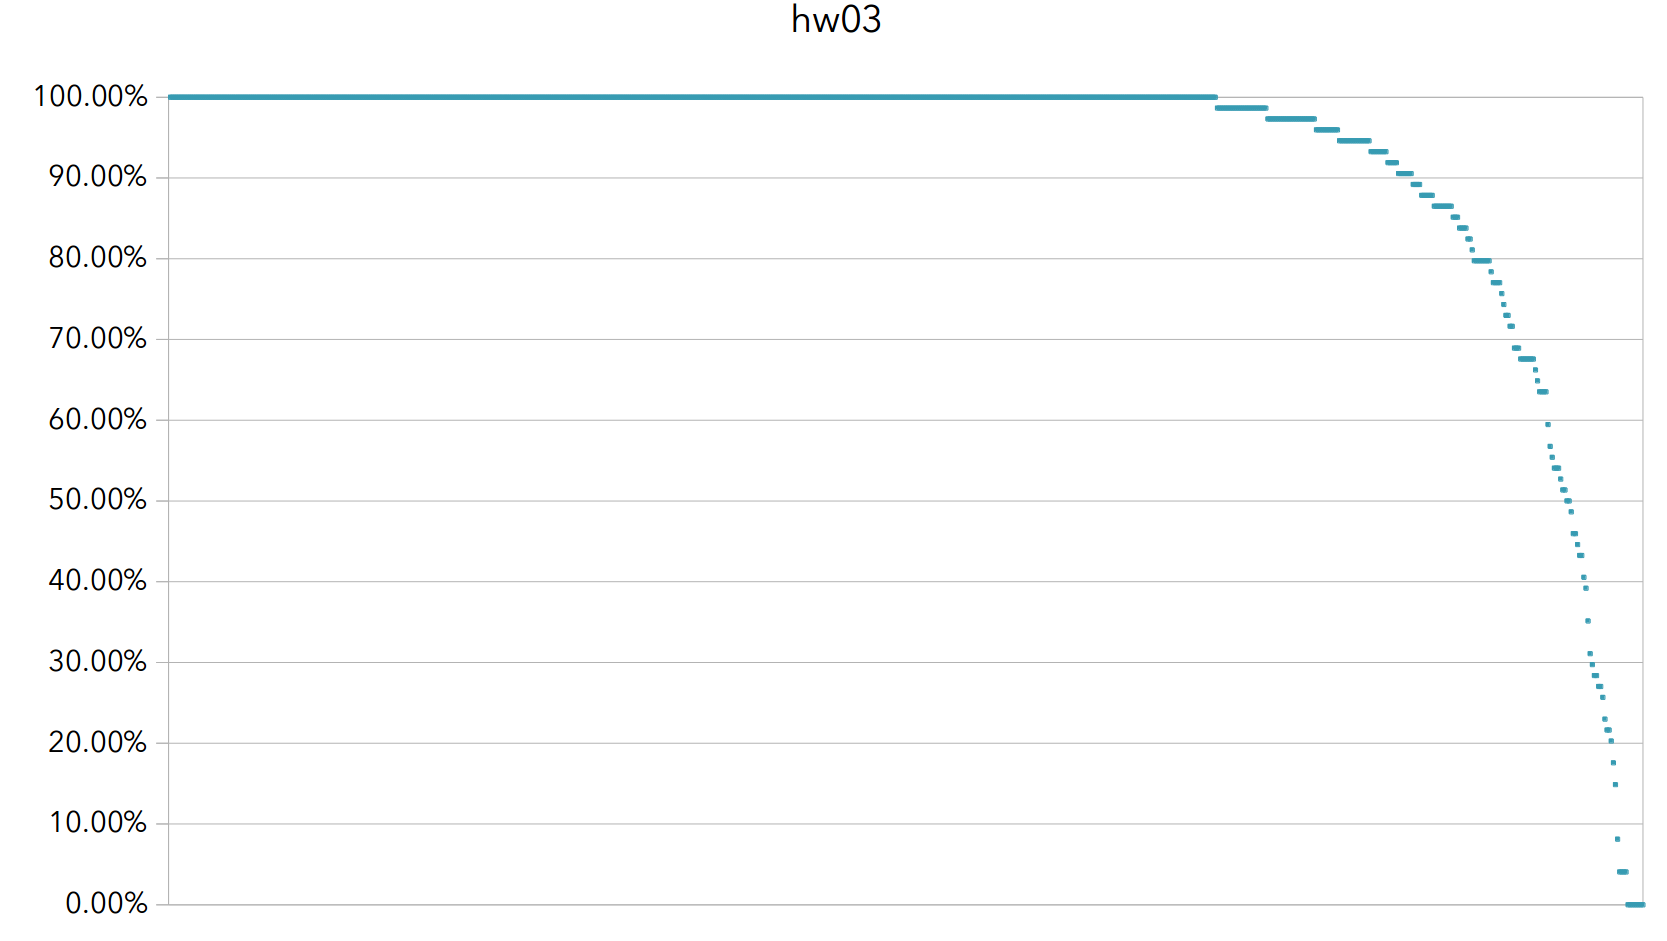
\includegraphics[width=0.8\textwidth]{./img/hw03-grades.png} %\pause
  \begin{enumerate}
  \myitem  Go to office hours! %\pause
  \myitem  I'll hw03 move to basis out of 70 (instead of 74). %\pause
  \myitem  Will be some opportunity for extra credit later.
  \end{enumerate}
\end{frame}

%%%%%%%%%%%%%%%%%%%%%%%%%%%%%%%%%%%%%%%%%%%%%%%%%%%%%%%%%%%%%%%%%%%%%%%%%%%%%%%%
\begin{frame}[fragile]
  \frametitle{Homework}
  \Enlarge

  Clunker Motors Inc. is recalling all vehicles in its Extravagant line from model years 1999-2002 as well all vehicles in its Guzzler line from model years 2004-2007.

  Given variables \texttt{modelYear} and \texttt{modelName} write a statement that assigns \texttt{True} to \texttt{recalled} if the values of \texttt{modelYear} and \texttt{modelName} match the recall details and assigns \texttt{False} otherwise.
\end{frame}

%%%%%%%%%%%%%%%%%%%%%%%%%%%%%%%%%%%%%%%%%%%%%%%%%%%%%%%%%%%%%%%%%%%%%%%%%%%%%%%%
\begin{frame}[fragile]
  \frametitle{Homework}
  \Enlarge

  Clunker Motors Inc. is recalling all vehicles in its Extravagant line from model years 1999-2002. Given a variable \texttt{modelYear} and a string \texttt{modelName} write a statement that prints the message \texttt{"RECALL"} to standard output if the values of \texttt{modelYear} and \texttt{modelName} match the recall details.
\end{frame}

%%%%%%%%%%%%%%%%%%%%%%%%%%%%%%%%%%%%%%%%%%%%%%%%%%%%%%%%%%%%%%%%%%%%%%%%%%%%%%%%
\begin{frame}[fragile]
  \frametitle{Homework}
  \Enlarge

  Assume that \texttt{x} is a string variable which has been given a value. Write an expression whose value is \texttt{True} if and only if \texttt{x} is alphanumeric, that is, either a letter or a decimal digit.
\end{frame}

%%%%%%%%%%%%%%%%%%%%%%%%%%%%%%%%%%%%%%%%%%%%%%%%%%%%%%%%%%%%%%%%%%%%%%%%%%%%%%%%
\section{Conditional Execution}

%%%%%%%%%%%%%%%%%%%%%%%%%%%%%%%%%%%%%%%%%%%%%%%%%%%%%%%%%%%%%%%%%%%%%%%%%%%%%%%%
\begin{frame}[fragile]
  \frametitle{Example:  \texttt{if} statement}
  \Enlarge

  \begin{semiverbatim}
ans = input( "Enter a number:" )
if float(ans) < 0:
    print( "The number was negative." )
  \end{semiverbatim}
\end{frame}

%%%%%%%%%%%%%%%%%%%%%%%%%%%%%%%%%%%%%%%%%%%%%%%%%%%%%%%%%%%%%%%%%%%%%%%%%%%%%%%%
\begin{frame}[fragile]
  \frametitle{Control flow}
  \Enlarge

  \begin{itemize}
  \myitem  \emph{Control flow} represents actual sequence of lines executed by processor. %\pause
  \myitem  \emph{Conditional execution} lets you execute (or not) a block of code based on logical comparison.
  \end{itemize}
\end{frame}

%%%%%%%%%%%%%%%%%%%%%%%%%%%%%%%%%%%%%%%%%%%%%%%%%%%%%%%%%%%%%%%%%%%%%%%%%%%%%%%%
\begin{frame}[fragile]
  \frametitle{Branched control flow}
  \Enlarge

  \begin{itemize}
  \myitem  We often need to make decisions with \emph{several} options. %\pause
  \myitem  \emph{Branched conditional execution} lets you execute one of several blocks of code.
  \end{itemize}
\end{frame}

%%%%%%%%%%%%%%%%%%%%%%%%%%%%%%%%%%%%%%%%%%%%%%%%%%%%%%%%%%%%%%%%%%%%%%%%%%%%%%%%
\begin{frame}[fragile]
  \frametitle{Example}
  \Enlarge

  \begin{semiverbatim}
def absolute(x):
    if x >= 0:
        return x
    else:
        return -x
  \end{semiverbatim}
\end{frame}

%%%%%%%%%%%%%%%%%%%%%%%%%%%%%%%%%%%%%%%%%%%%%%%%%%%%%%%%%%%%%%%%%%%%%%%%%%%%%%%%
\begin{frame}[fragile]
  \frametitle{\texttt{if}/\texttt{else} statement}
  \Enlarge

  \begin{itemize}
  \myitem  We create an \texttt{if}/\text{else} statement as follows:
    \begin{itemize}
    \mysubitem  the keyword \texttt{if}
    \mysubitem  a logical comparison (results in \texttt{bool})
    \mysubitem  a \textbf{block} of code
    \mysubitem  the keyword \texttt{else}
    \mysubitem  a different \textbf{block} of code
    \end{itemize}
  \end{itemize}
\end{frame}

%%%%%%%%%%%%%%%%%%%%%%%%%%%%%%%%%%%%%%%%%%%%%%%%%%%%%%%%%%%%%%%%%%%%%%%%%%%%%%%%
\begin{frame}[fragile]
  \frametitle{Sequence operators}
  \Enlarge

  \begin{itemize}
  \myitem  These produce Boolean output.
    \begin{tabular}{ll}
    \texttt{in}     & Is one string inside of the other? \\
    \texttt{not in} & Is one string not inside of the other?
    \end{tabular}
  \end{itemize}
\end{frame}

%%%%%%%%%%%%%%%%%%%%%%%%%%%%%%%%%%%%%%%%%%%%%%%%%%%%%%%%%%%%%%%%%%%%%%%%%%%%%%%%
\begin{frame}[fragile]
  \frametitle{Example}
  \Enlarge

  \begin{semiverbatim}
def fun(s):
    return s.isalpha() and 'a' in s

x = fun( "sam" ) and fun( "AS" )
  \end{semiverbatim}
  What is the value of \texttt{x}?
  \begin{enumerate}[label=\Alph*]
  \item  \texttt{True}
  \item  \texttt{False}  $\star$
  \end{enumerate}
\end{frame}

%%%%%%%%%%%%%%%%%%%%%%%%%%%%%%%%%%%%%%%%%%%%%%%%%%%%%%%%%%%%%%%%%%%%%%%%%%%%%%%%
\begin{frame}[fragile]
  \frametitle{Nesting}
  \Enlarge

  \begin{itemize}
  \myitem  Sometimes we need to make more than one decision. %\pause
  \myitem  We can \emph{nest} blocks. %\pause
    \begin{Verbatim}
word = input( 'Enter a Scrabble word:  ' )
if not word.isalpha():
    print( 'There are only letters in Scrabble!' ) %\pause
else:
    if not word.isupper():      # why not
                                # `word.islower()`?
        word = word.upper()
    print( 'You entered %s.' % word )
    \end{Verbatim}
  \end{itemize}
\end{frame}

%%%%%%%%%%%%%%%%%%%%%%%%%%%%%%%%%%%%%%%%%%%%%%%%%%%%%%%%%%%%%%%%%%%%%%%%%%%%%%%%
\begin{frame}
  \frametitle{Nesting}
  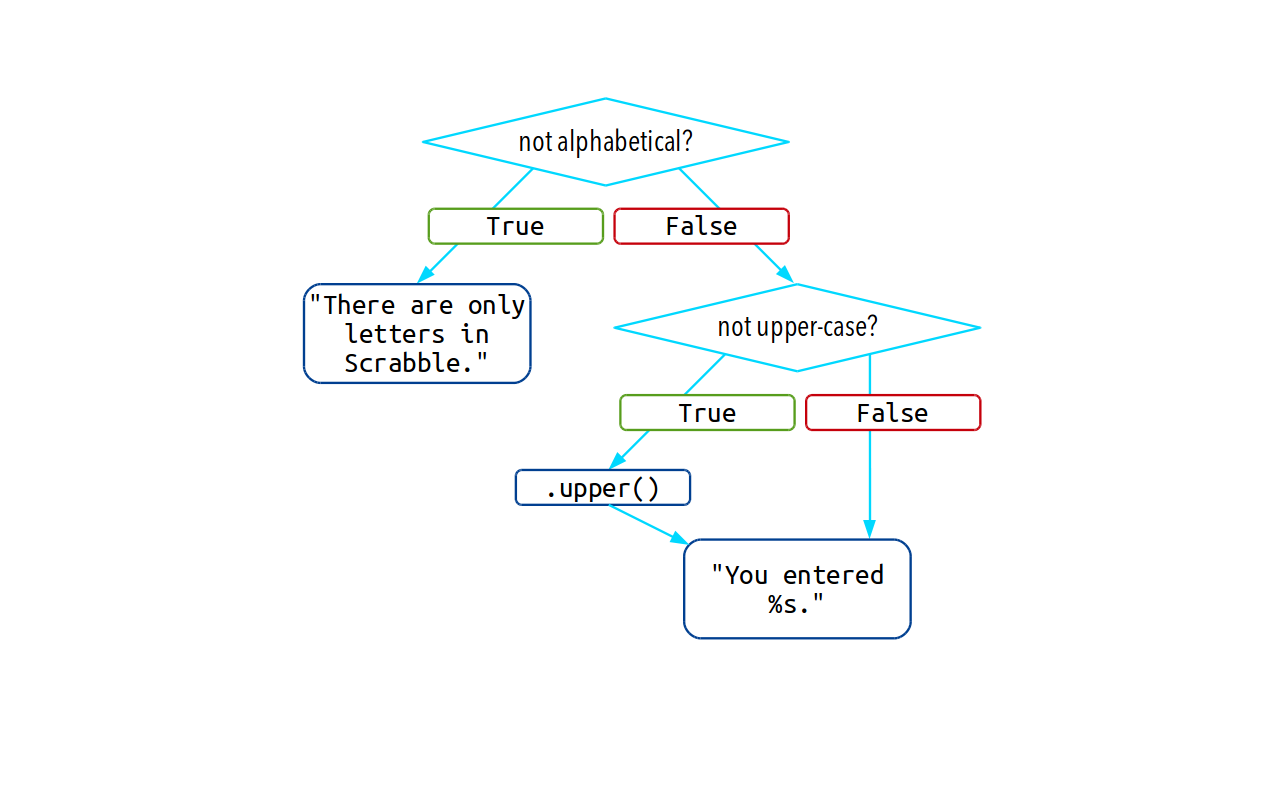
\includegraphics[width=\textwidth]{./img/control-flow-nesting-else.png}
\end{frame}

%%%%%%%%%%%%%%%%%%%%%%%%%%%%%%%%%%%%%%%%%%%%%%%%%%%%%%%%%%%%%%%%%%%%%%%%%%%%%%%%
\begin{frame}
  \frametitle{Exercise:  Nesting}
  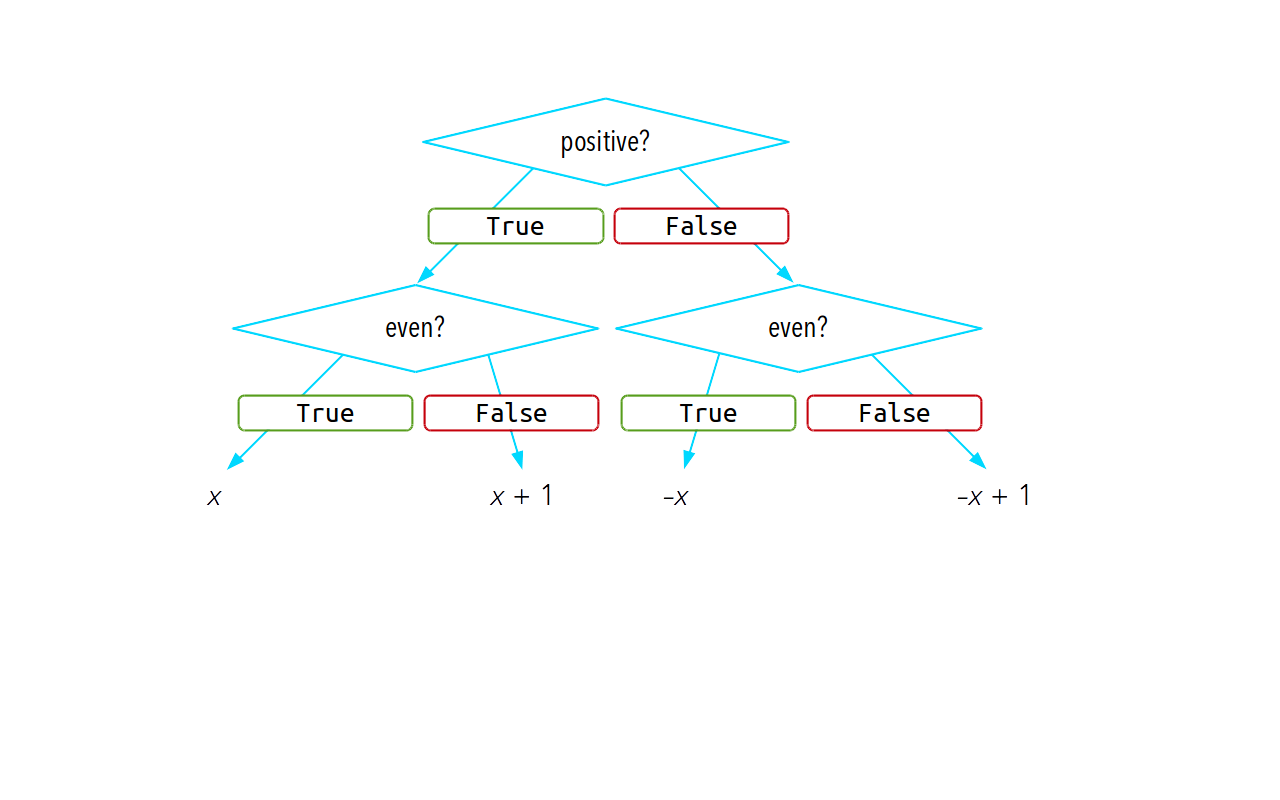
\includegraphics[width=\textwidth]{./img/control-flow-nesting-else-ex.png}
\end{frame}

%%%%%%%%%%%%%%%%%%%%%%%%%%%%%%%%%%%%%%%%%%%%%%%%%%%%%%%%%%%%%%%%%%%%%%%%%%%%%%%%
\begin{frame}[fragile]
  \frametitle{Example}
  \Enlarge

  \begin{semiverbatim}
def evenpos(x):
    if x >= 0:
        if (x%2) == 0:
            return x
        else:
            return x + 1
    else:
        if (x%2) == 0:
            return -x
        else:
            return (-x) + 1
  \end{semiverbatim}
\end{frame}

%%%%%%%%%%%%%%%%%%%%%%%%%%%%%%%%%%%%%%%%%%%%%%%%%%%%%%%%%%%%%%%%%%%%%%%%%%%%%%%%
\begin{frame}[fragile]
  \frametitle{Multi-way branch}
  \Enlarge

  \begin{itemize}
  \myitem  Sometimes we need to select among many choices.
  \end{itemize}
  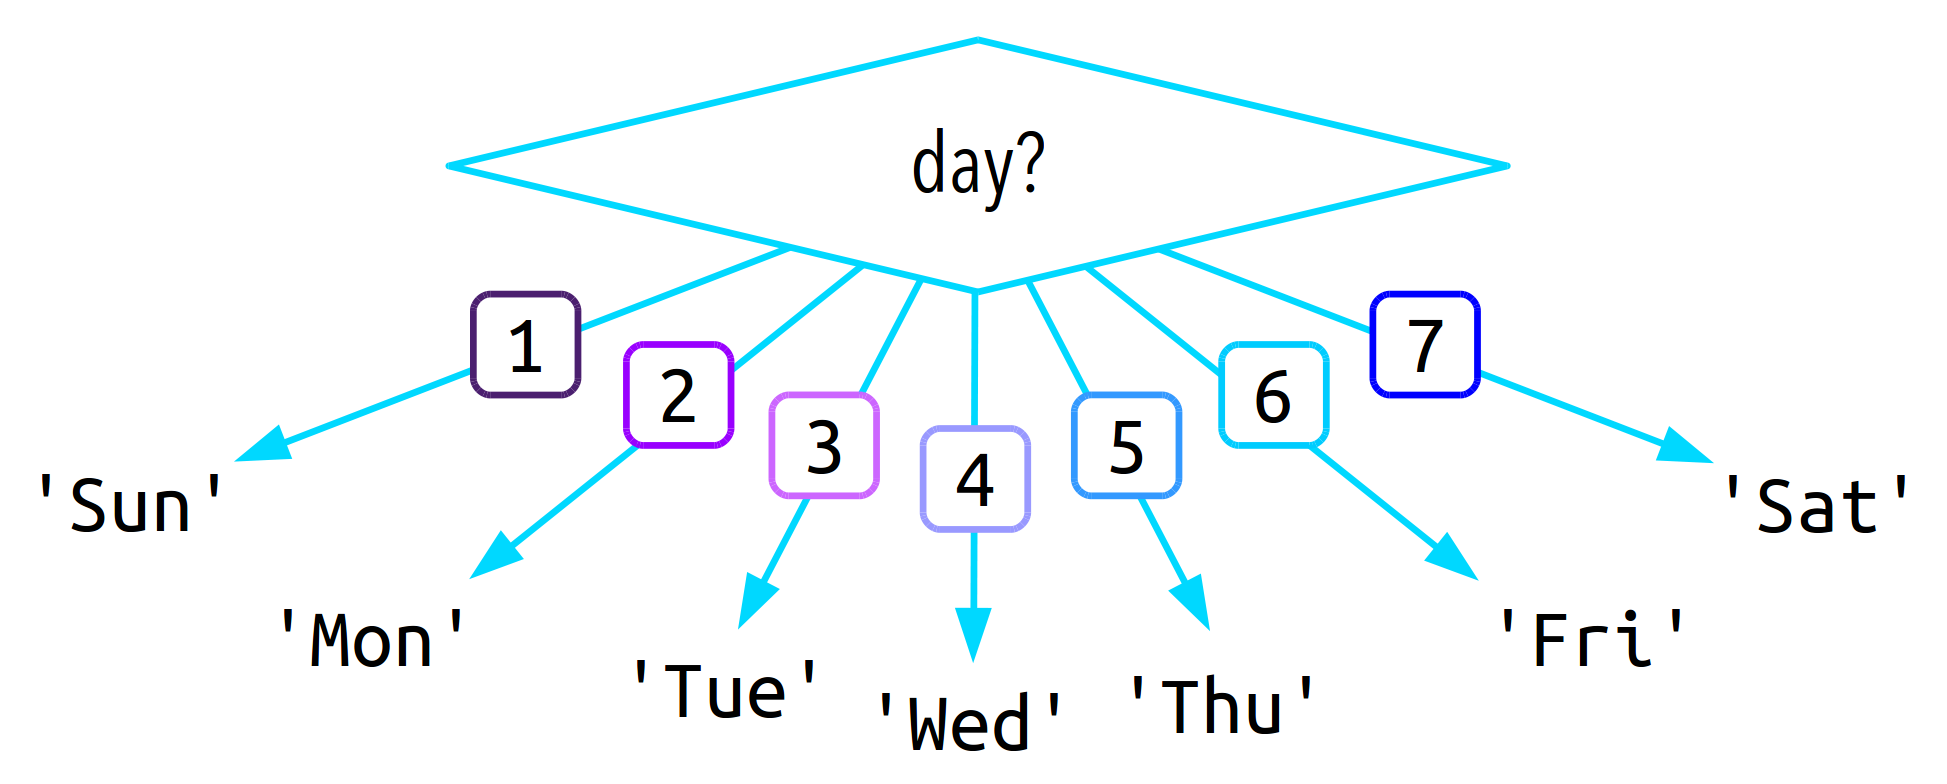
\includegraphics[width=0.8\textwidth]{./img/control-flow-multi.png}
\end{frame}

%%%%%%%%%%%%%%%%%%%%%%%%%%%%%%%%%%%%%%%%%%%%%%%%%%%%%%%%%%%%%%%%%%%%%%%%%%%%%%%%
\begin{frame}[fragile]
  \frametitle{Example}
  \Enlarge

  \begin{semiverbatim}
if day == 1:
    print("Sunday")
else:
    if day == 2:
        print("Monday")
    else:
        if day == 3:
            print("Tuesday")
        else:
            if day == 4:
                print("Wednesday")
            else:
                if day == 5:
                    print("Thursday")
                else:
                    if day == 6:
                        print("Friday")
                    else:
                        if day == 7:
                            print("Saturday")
  \end{semiverbatim}
\end{frame}

%%%%%%%%%%%%%%%%%%%%%%%%%%%%%%%%%%%%%%%%%%%%%%%%%%%%%%%%%%%%%%%%%%%%%%%%%%%%%%%%
\begin{frame}[fragile]
  \frametitle{Example}
  \Enlarge

  \begin{semiverbatim}
if day == 1:
    print("Sunday")
elif day == 2:
    print("Monday")
elif day == 3:
    print("Tuesday")
elif day == 4:
    print("Wednesday")
elif day == 5:
    print("Thursday")
elif day == 6:
    print("Friday")
elif day == 7:
    print("Saturday")
else:
    print("That is not a valid day.")
  \end{semiverbatim}
\end{frame}

%%%%%%%%%%%%%%%%%%%%%%%%%%%%%%%%%%%%%%%%%%%%%%%%%%%%%%%%%%%%%%%%%%%%%%%%%%%%%%%%
\begin{frame}[fragile]
  \frametitle{\texttt{if}/\texttt{elif}/\texttt{else} statement}
  \Enlarge

  \begin{itemize}
  \myitem  We create an \texttt{if}/\texttt{elif}/\texttt{else} statement as follows:
    \begin{itemize}
    \mysubitem  the keyword \texttt{if}
    \mysubitem  a logical comparison (results in \texttt{bool})
    \mysubitem  a \textbf{block} of code
    \mysubitem  the keyword \texttt{elif}
    \mysubitem  a logical comparison (results in \texttt{bool})
    \mysubitem  a \textbf{block} of code
    \mysubitem  the keyword \texttt{else}
    \mysubitem  a different \textbf{block} of code
    \end{itemize}
  \end{itemize}
\end{frame}

%%%%%%%%%%%%%%%%%%%%%%%%%%%%%%%%%%%%%%%%%%%%%%%%%%%%%%%%%%%%%%%%%%%%%%%%%%%%%%%%
\section{Iteration Redux}

%%%%%%%%%%%%%%%%%%%%%%%%%%%%%%%%%%%%%%%%%%%%%%%%%%%%%%%%%%%%%%%%%%%%%%%%%%%%%%%%
\begin{frame}[fragile]
  \frametitle{Example}
  \Enlarge

  \begin{semiverbatim}
colors = [ 'red', 'yellow', 'blue',
           'jale', 'ulfire' ]
for color in colors:
    print( color )
  \end{semiverbatim}
\end{frame}

%%%%%%%%%%%%%%%%%%%%%%%%%%%%%%%%%%%%%%%%%%%%%%%%%%%%%%%%%%%%%%%%%%%%%%%%%%%%%%%%
\begin{frame}[fragile]
  \frametitle{Defining loops:  \texttt{for}}
  \Enlarge

  \begin{itemize}
  \myitem  A \texttt{for} loop requires:
    \begin{itemize}
    \mysubitem  the keyword \texttt{for}
    \mysubitem  a loop variable
    \mysubitem  the keyword \texttt{in}
    \mysubitem  a set of values
    \mysubitem  a \textbf{block} of code
    \end{itemize}
  \myitem  \texttt{for} loops iterate over \emph{iterable} types one at a time.
  \end{itemize}
\end{frame}

%%%%%%%%%%%%%%%%%%%%%%%%%%%%%%%%%%%%%%%%%%%%%%%%%%%%%%%%%%%%%%%%%%%%%%%%%%%%%%%%
\begin{frame}[fragile]
  \frametitle{Example}
  \Enlarge

  \begin{semiverbatim}
s = 'abcdefg'
t = ''
for c in s:
    t = c + t
  \end{semiverbatim}
  What is the value of \texttt{t}?
  \begin{enumerate}[label=\Alph*]
  \item  \texttt{'abcdefg'}
  \item  \texttt{'gfedcba'}
  \item  \texttt{'a'}
  \item  \texttt{'g'}
  \end{enumerate}
\end{frame}

%%%%%%%%%%%%%%%%%%%%%%%%%%%%%%%%%%%%%%%%%%%%%%%%%%%%%%%%%%%%%%%%%%%%%%%%%%%%%%%%
\begin{frame}[fragile]
  \frametitle{Exercise}
  \Enlarge

  Write a function to sum all of the digits in a number.  \emph{I.e.},

  \begin{center}
  \texttt{12145} $\rightarrow$ \texttt{1 + 2 + 1 + 4 + 5} $\rightarrow$ \texttt{13}
  \end{center}
\end{frame}

%%%%%%%%%%%%%%%%%%%%%%%%%%%%%%%%%%%%%%%%%%%%%%%%%%%%%%%%%%%%%%%%%%%%%%%%%%%%%%%%
\begin{frame}[fragile]
  \frametitle{Solution (\texttt{for})}
  \Enlarge

  \begin{semiverbatim}
def sum_digits( n ):
    result = 0
    for letter in str( n ):
        result += int( letter )
    return result
  \end{semiverbatim}
\end{frame}

%%%%%%%%%%%%%%%%%%%%%%%%%%%%%%%%%%%%%%%%%%%%%%%%%%%%%%%%%%%%%%%%%%%%%%%%%%%%%%%%
\begin{frame}[fragile]
  \frametitle{Example}
  \Enlarge

  \begin{semiverbatim}
for i in range(10):
    print(i ** 2)
  \end{semiverbatim}
\end{frame}

%%%%%%%%%%%%%%%%%%%%%%%%%%%%%%%%%%%%%%%%%%%%%%%%%%%%%%%%%%%%%%%%%%%%%%%%%%%%%%%%
\begin{frame}[fragile]
  \frametitle{\texttt{range} function}
  \Enlarge

  \begin{itemize}
  \myitem  The \texttt{range} function returns an \texttt{iterator} containing integers. %\pause
  \myitem  \texttt{range} can be cast as a \texttt{list}. %\pause
  \myitem  Two arguments:
    \begin{itemize}
    \mysubitem  (optional) the starting value of the range (inclusive)
    \mysubitem  the ending value of the range (exclusive)
    \end{itemize}
  \end{itemize}
\end{frame}

%%%%%%%%%%%%%%%%%%%%%%%%%%%%%%%%%%%%%%%%%%%%%%%%%%%%%%%%%%%%%%%%%%%%%%%%%%%%%%%%
\section{Reminders}

%%%%%%%%%%%%%%%%%%%%%%%%%%%%%%%%%%%%%%%%%%%%%%%%%%%%%%%%%%%%%%%%%%%%%%%%%%%%%%%%
\begin{frame}
  \frametitle{Reminders}
  \Enlarge

  \begin{itemize}
  \myitem  Homework \#4 is due Friday Sep.\ 23.
  \myitem  Midterm \#1 will be Monday Oct.\ 3.  (evening)
  \end{itemize}
\end{frame}

\end{document}
